\chapter{Excommunication}

When someone goes against the church's teachings and openly oppose the church and its
leaders, they can be excommunicated from the LDS Church. Figure \ref{fig:ex1} is an 
example of such:

\begin{figure}[h!]
  \centering
  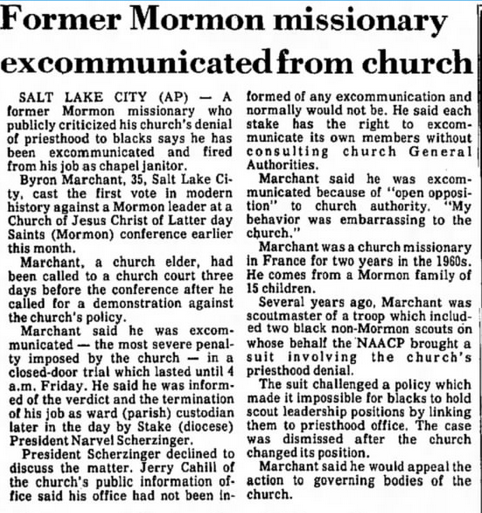
\includegraphics[width=0.4\linewidth]{articles/images/ex.png}
  \caption{The Daily Reporter (Dover, Ohio) 15 Oct 1977}
  \label{fig:ex1}
\end{figure}

In the early days of the church, leaders were known to excommunicate followers more
often and loose. It has slowed down a bit as church goers have gotten in line as it
were. But there are still excommunications which happen every year. Of course, not 
all end up in the newspaper like Figure \ref{fig:ex1}. But it still happens.

It was said during the succession crisis of 1844 after Joseph Smith died, anyone who
voted against Brigham Young were excommunicated. Even though a vote for and against
was called for. Anytime a person in the church votes against or opposing the leadders
of the church, they are in danger of apostasy.

To face excommunication from the church, you are taken off the roles of the church.
Your baptism becomes null and void, any temple blessings are revoked. You are not
able to speak in a church meeting, give a prayer, take the sacrament or participate
in any way at all.

Some people are shunned by their family members. This is not a church teaching to be
shunned, but it does happen. Family can't accept that one would not want to follow a
church they grew up in. They cannot understand how a person would abandon their God
as it were.

I think that's a main issue poeple don't understand. Just because a person is
excommunicated from the church, it doesn't mean they have lost faith in Christ and a
belief in God. Perhaps they have come to understand Christ a little bit more than
they did when in the LDS faith.

The leaders say it's to help the repentence process, to help others come back to the
church and to accept Christ's atonement in their lives. In effect, the church will
not leave them alone. If a person is openly opposing church leaders, maybe they want
to be left alone. It's a thought.

Members ask all the time to be left alone from the church, yet because the member is
on the role the church continues to visit the member. The only way to avoid any of
this is to either be excommunicated or to request your name be removed from the
records of the church.

Even removing your name isn't an easy process. The bishop of the local ward will
still want to see if there's anything they can do to help you come back to the fold.
It's a never ending process which constantly loops over again.

It's sad to think about.

In a talk given to the All-Church Coordinating Council, Boyd K. Packer said the
following:

\begin{displayquote}
There are three areas where members of the Church, influenced by social and political 
unrest, are being caught up and led away. I chose these three because they have made 
major invasions into the membership of the Church. In each, the temptation is for us 
to turn about and face the wrong way, and it is hard to resist, for doing it seems 
so reasonable and right.

The dangers I speak of come from the gay-lesbian movement, the feminist movement 
(both of which are relatively new), and the ever-present challenge from the so-called 
scholars or intellectuals.\footnote{Talk to the All-Church Coordinating Council,
Elder Boyd K. Packer, May 18, 1993}
\end{displayquote}

If a person in the church identifies with any of these three, they can face church
discipline. That may come in the form of excommunication, or the lesser judgement of
disfellowship.

To openly think for yourself goes against church teachings. You are to obey the
commandments the church has laid out, which they claim come from the Lord. Only then
will you be able to be in full fellowship with the Church of Chirst. Any deviation
from this path and you are facing dangerous waters.

In the same breath LDS faithful are taught to seek out learning and to seek things
which are good. They are taught to seek if something is right or not. To not blindly
follow a prophet of God but to learn for themselves if the teachings are true. Once
they learn if it is true or false they can come to a decision.

But if you decided what a prophet of God has spoken to be false, you are on thin ice
and there is no real coming back from that. The official statment is the church must
protect its good name.\footnote{
The purposes of disciplinary councils are to save the souls of transgressors, 
protect the innocent, and safeguard the purity, integrity, 
and good name of the Church.
https://www.lds.org/topics/church-disciplinary-councils?lang=eng
}

So, does that mean forget about the people who are trying to learn from the best
books and who might bring about history issues? Who are simply trying to understand
the religion they have believed in their whole life? There's a lot to be said about
the church's history, not all is good mind you. There is a lot to be said about all
of it. Choosing what you want to believe to be true and what is true? That's not how
any of this works.

Jesus cared more about the people then he did protecting a church. Even when Saul was
persecuting the church, Jesus appeared to him (it still isn't clear which way Jesus
appeared to Saul, be it visual or audio\footnote{Acts 9:7; Acts 22:9}), 
and Saul changed his ways. Jesus was concerned about Saul and the people, the people 
Saul was persecuting. Jesus didn't care about the ``good name of the church", He 
cared about the people.

Back to the image about the man who was excommunicated due to him being outspoken
about blacks receiving the priesthood. The newspaper article was October 1977, less
than a year before the June 1978 ``revelation". He knew what was right, he knew what
needed to be done. But because he went against the church's established doctrine and
policy, he was excommunicated. The church would later change their minds about black
people and the priesthood etc. as already mentioned in another article, but to go
against someone for pressing for that which is right? Doesn't seem logical.

A person does not seek out excommunication from the church. They desire to embrace
the church and help grow it and move it forward. Sometimes their way of thinking
tends to squeeze the church where the leaders think it ought not to be squeezed and
that person must be silenced. Thus an excommunication occurs.

Back in the day, they would even put on display those who had been excommunicated
including their wards and stakes they came from\footnote{Improvement Era, June 1945, 
Vol 48 No 6, Page 345.}. Some would even have to get up at the pulpit and tell of 
their wrongdoings as part of their repentance process.